%
% File acl-hlt2011.tex
%
% Contact: gdzhou@suda.edu.cn
%%
%% Based on the style files for ACL2008 by Joakim Nivre and Noah Smith
%% and that of ACL2010 by Jing-Shin Chang and Philipp Koehn

\documentclass[11pt]{article}
\usepackage{acl-hlt2011}
\usepackage{times}
\usepackage{latexsym}
\usepackage{amsmath}
\usepackage{multirow}
%\usepackage{fullpage}
\usepackage{url}
\usepackage{color}
\usepackage{colortbl}
\usepackage[vlined,figure]{algorithm2e}
\usepackage{graphicx} 



\DeclareMathOperator*{\argmax}{arg\,max}

\definecolor{red}{rgb}{1,0,0}
\definecolor{lightgray}{cmyk}{0,0,0,.08}

\newcommand{\mnote}[1]{\marginpar{%
  \vskip-\baselineskip
  \raggedright\footnotesize
  \itshape\hrule\smallskip\tiny{#1}\par\smallskip\hrule}}  

%\newcommand{\mtodo}[1]{}
\newcommand{\mtodo}[1]{\mnote{\textcolor{red}{#1}}}
\newcommand{\red}[1]{\textcolor{red}{#1}}
\newcommand{\todo}[1]{\textcolor{red}{TODO: #1}}
\newcommand{\todop}[2]{\noindent\textcolor{red}{TODO for #1:} #2\\}
\newcommand{\todopi}[2]{[\textcolor{red}{TODO for #1:} #2]}
\newcommand{\secref}[1]{Section~\ref{#1}}
\newcommand{\tabref}[1]{Table~\ref{#1}}
\newcommand{\figref}[1]{Figure~\ref{#1}}
\newcommand{\code}[1]{{\small \tt #1}}
\newcommand{\emq}[1]{\emph{``#1''}}
\newcommand{\paraheader}[1]{\vskip 0.05in \noindent\emph{#1}}
\newcommand{\skipheader}{\vskip 0.05in}

\newcommand{\bm}{\boldsymbol}
\def\bs#1{\boldsymbol{#1}}

\newenvironment{my_itemize}{
\begin{itemize}
  \setlength{\itemsep}{2pt}
  \setlength{\parskip}{2pt}
  \setlength{\parsep}{1pt}}{\end{itemize}
}

%\setlength\titlebox{6.5cm}    % Expanding the titlebox
\setlength\titlebox{3.75cm}    % Expanding the titlebox

\title{Toward Statistical Machine Translation without Parallel Corpora}

\author{}
 \author{Alex Klementiev \ \ \ \  Ann Irvine \ \ \ \ Chris Callison-Burch \ \ \ \ David Yarowsky \\
 Center for Language and Speech Processing \\ Johns Hopkins University}
\date{}

\begin{document}
\maketitle
\begin{abstract}
%The parameters of statistical translation models are typically estimated from large bilingual parallel corpora.  However, these resources  are not available for most language pairs and are expensive to produce from scratch.  In this work, 
We estimate the parameters of a phrase-based statistical machine translation system from 
%cheap 
\emph{monolingual} corpora instead of a \emph{bilingual} parallel corpus.  We extend existing research on bilingual lexicon induction to estimate lexical and phrasal translation probabilities for MT scale phrase-tables. We propose a novel algorithm to estimate re-ordering probabilities from monolingual data. We report translation results for an end-to-end translation system using these monolingual features alone.  In principle, our method only requires two large monolingual corpora, a small bilingual dictionary, and a small bitext for tuning feature weights.  In this paper, we examine an idealization where a phrase-table is given.  We examine the degradation in translation performance when bilingually estimated translation probabilities are removed, and show that 80\%+ of the loss can be recovered with monolingually estimated features alone.  We further show that our monolingual features add 1.5 BLEU points when combined with standard bilingually estimated phrase table features. 
% We perform a feature lesion study that shows how much translation performance decreases when parameters estimated from bitext are removed and how much of that loss can be restored when monolingually-estimated equivalents are added.  We show that more than 81\% of the loss can be recovered with monolingual data alone.  We also show that the monolingual features we introduce account for about 1.5 BLEU point gain when added to the standard phrase-based pipeline.

% Large volumes of parallel text are required before translation models produce high quality translations, but sufficiently large corpora are available for  very few language pairs.  On the other hand, monolingual data is widely available and cheap to collect.  In this work, we propose a set of cues derived from monolingual resources and systematically introduce them in a phrase-based machine translation pipeline \emph{in place} of features induced from parallel data.  We show on two language pairs that monolingual data can take us a long way toward  inducing a high quality machine translation system.

%The parameters of statistical translation models of are estimated from bilingual parallel corpora.    Large volumes of parallel text are required before translation models produce high quality translations, but sufficiently large corpora are available for  very few language pairs.  On the other hand, monolingual data is widely available and cheap to collect.  In this work, we propose a set of cues derived from monolingual resources and systematically introduce them in a phrase-based machine translation pipeline \emph{in place} of features induced from parallel data.  We show on two language pairs that monolingual data can take us a long way toward  inducing a high quality machine translation system.

%Current statistical machine translation methods rely on very large parallel corpora to achieve state of the art performance.  However, such resources are only available for very few language pairs as they are very expensive to obtain.  On the other hand, monolingual data (such as newswire) is widely available and cheap to collect.  In this work, we propose a set of cues derived from monolingual resources and systematically introduce them in a phrase-based machine translation pipeline \emph{in place} of features induced from parallel data.  We show on two language pairs that monolingual data can take us a long way toward  inducing a high quality machine translation system.\mtodo{Need a more concrete statement.}
\end{abstract}

% ------------------------------------------------

\vspace{-.5cm}
\section{Introduction} \label{sect:intro}

The parameters of statistical models of translation are typically estimated from large bilingual parallel corpora \cite{Brown:1993}.  However, these resources are not available for most language pairs and they are expensive to produce in quantities sufficient for building a good translation system \cite{Germann2001}.
We attempt an entirely different approach: we use cheap and plentiful monolingual resources to induce an end-to-end statistical machine translation system.  In particular, we extend the long line of work on inducing translation lexicons (beginning with \newcite{Rapp:1995}) and propose to use multiple independent cues present in monolingual texts to estimate lexical and phrasal translation probabilities for large, MT-scale phrase-tables.  We then introduce a novel algorithm to estimate reordering features from monolingual data alone, and report the performance of a phrase-based statistical model \cite{Koehn:2003} estimated on these monolingual features.

Most of the prior work on lexicon induction is motivated by the idea that it could be applied to machine translation but stops short of actually doing so.  Lexicon induction holds the potential to create machine translation systems for languages which do not have extensive parallel corpora.  Training would only require two large monolingual corpora and a small bilingual dictionary, if one is available.  The idea is that intrinsic properties of monolingual data (possibly along with a handful of bilingual pairs to act as example mappings) can provide independent but informative cues to learn translations, because words (and phrases) behave similarly across languages.  This work is the first attempt to extend and apply these ideas to an end-to-end machine translation pipeline.  While we make an explicit assumption that a table of phrasal translations is given a priori, we induce every other parameter of a full phrase-based translation system from monolingual data alone.  The contributions of this work are:

%\todop{Chris}{Now that we have an Urdu experiment, we should emphasize it in text / in the list below / in the abstract?}
%\todop{Chris}{Motivate the "no parallel data" setting (e.g. from commented out text?) here and possibly in the abstract.}
%\todop{Chris}{Add a bullet that we are publishing data? Will also mention it in the \secref{sect:exp}.}
%Current statistical machine translation (SMT) methods (e.g. \cite{Koehn:2003,Chiang:2005}) crucially rely on vast amounts of sentence aligned translations in order to achieve state of the art performance.  These resources are only available for very few language pairs because producing them in sufficient quantities is an expensive and time consuming endeavor.  Moreover, the SMT system performance tends to drop if test data comes from a different domain then the parallel data used in training\mtodo{Need a good MT adaptation reference}.  

%The rest of the paper is organized as follows.  \secref{sect:bckg} begins with the relevant background on the phrase-based SMT framework we will use in the rest of the paper and continues to give a brief overview of the existing work on inducing translation lexicons. \secref{sect:mono} motivates and introduces translation and reordering features induced from monolingual data alone.   \secref{sect:exp} studies the informativeness of these features as they are added to the Machine Translation pipeline.  Finally, \secref{sect:conc} concludes and discusses directions for future work.

\begin{itemize}
  \item In \secref{sect:bckg:lexind} we analyze the challenges of using bilingual lexicon induction for statistical MT (performance on low frequency items, and moving from words to phrases).
  \item In Sections \ref{sect:phrasalfeats} and \ref{sect:lexfeats} we use multiple cues present in monolingual data to estimate lexical and phrasal translation scores.
  \item In \secref{sect:order} we propose a novel algorithm for estimating phrase reordering features from monolingual texts.
  \item Finally, in \secref{sect:results} we systematically drop  feature functions  from a phrase table and then replace with monolingually estimated equivalents, reporting end-to-end translation quality.
  % with a fixed phrase-table with monolingually estimated parameters. 
\end{itemize}

%Current statistical machine translation (SMT) methods (e.g. \cite{Koehn:2003,Chiang:2005}) crucially rely on vast amounts of sentence aligned translations in order to achieve state of the art performance.  These resources are only available for very few language pairs because producing them in sufficient quantities is an expensive and time consuming endeavor.  Moreover, the SMT system performance tends to drop if test data comes from a different domain then the parallel data used in training\mtodo{Need a good MT adaptation reference}.  


% ------------------------------------------------
% \section{Related Work} \label{sect:related-work}
% ccb - moved related work the end.


% ------------------------------------------------

\section{Background} \label{sect:bckg}

We begin with a brief overview of the standard phrase-based statistical machine translation model do define the parameters we replace with monolingual alternatives.  We continue with a discussion of bilingual lexicon induction; we extend these methods to estimate the monolingual parameters in \secref{sect:mono}.   This approach allows us to replace expensive/rare bilingual parallel training data with two large monolingual corpora, a small bilingual dictionary, and $\approx$1,000 sentence bilingual development set, which are comparatively plentiful/inexpensive.

%We attempt to estimate the parameters of a phrase-based translation model (described in \ref{sect:bckg:smt}) using techniques from bilingual lexicon induction (\ref{sect:bckg:lexind}).  This allows us to replace expensive/rare bilingual parallel training data with  two large monolingual corpora, a small bilingual dictionary, and $\approx$1,000 sentence bilingual development set, which are comparatively plentiful/inexpensive.

%These parallel resources are only available for a small set of language pairs and are very expensive to compile in sufficient quantities.  
%In this work, we estimate the parameters of the phrase-based formalism from {\em monolingual} texts, which are much more plentiful. 

\subsection{Parameters of phrase-based SMT} \label{sect:bckg:smt}

Statistical machine translation (SMT) was first formulated as a series of probabilistic models that learn word-to-word correspondences from sentence-aligned bilingual parallel corpora \cite{Brown:1993}.  \nocite{Brown1988}
%
Current methods, including {\em phrase-based} \cite{Och:2002,Koehn:2003} and {\em hierarchical} models \cite{Chiang:2005}, typically start by word-aligning a bilingual parallel corpus \cite{Och2003}.  They extract multi-word phrases that are consistent with the Viterbi word alignments, and use these phrases to build new translations.    A variety of parameters are estimated using the bitexts.  Here we review the parameters of the standard phrase-based translation  model \cite{Moses}, which we will later show how to estimate using monolingual texts instead.  These parameters are:
\begin{my_itemize}
\item \emph{Phrase pairs}.  
Phrase extraction heuristics \cite{Venugopal2003,Tillmann2003,Och2004} produce a set of phrase pairs $(e, f)$ that are consistent with the word alignments.  
%We consider the inventory of phrase pairs (irrespective of their scores) to be a model parameter.  
In this paper we assume that the phrase pairs are given (without any scores), and we induce every other parameter of the phrase-based model from monolingual data.
%Creating this inventory from monolingual texts alone is a major challenge, and we leave it for future work.

\item \emph{Phrase translation probabilities}.  Each phrase pair has a list of associated feature functions (FFs).  These include phrase translation probabilities ${\phi(e|f)}$ and ${\phi(f|e)}$ which are  typically calculated via maximum likelihood estimation. 

\item \emph{Lexical weighting}.  Since MLE overestimates ${\phi}$ for phrase pairs with sparse counts, lexical weighting FFs are used to smooth.  Average word translation probabilities ${w(e_i|f_j)}$ are calculated via phrase-pair-internal word alignments.

\item \emph{Reordering model}.  Each $(e, f)$ also has reordering parameters $p_o(\textnormal{orientation}|f,e)$ which indicate the distribution of its orientation wrt the previously translated phrase. Orientations are {\it monotone, swap, discontinuous} \cite{tillman:2004:HLTNAACL,Kumar2004}, see \figref{fig:reorderfeats}. 

\item \emph{Other features}. Other typical features are n-gram language model scores and phrase penalty (which governs whether to use fewer longer phrases or more shorter phrases).  These are not bilingually estimated, so we can re-use them directly without modification. 
\end{my_itemize}

\noindent
The features are combined in a log linear model, and their weights are set through minimum error rate training \cite{Och2003c}.
%Log linear formulation:
%  \begin{eqnarray*}
 %   p(\mathbf{e} | \mathbf{f}) & \propto & \exp \sum_{i=1}^{n}{\lambda_i h_i (\mathbf{e}, \mathbf{f})} \label{log-linear-formulation}\\
 %   \hat{e} & = & \argmax_{e}{p(\mathbf{e} | \mathbf{f}) }
 % \end{eqnarray*}
We use the same log linear formulation and MERT but propose alternatives derived directly from monolingual data for all parameters except for the phrase pairs themselves. Our pipeline still requires a small bitext of approximately 1,000 sentences to use as a development set for parameter tuning via MERT.


\begin{figure}[t]
%\vskip 0.1in
\begin{center}
\vspace{-.35cm}
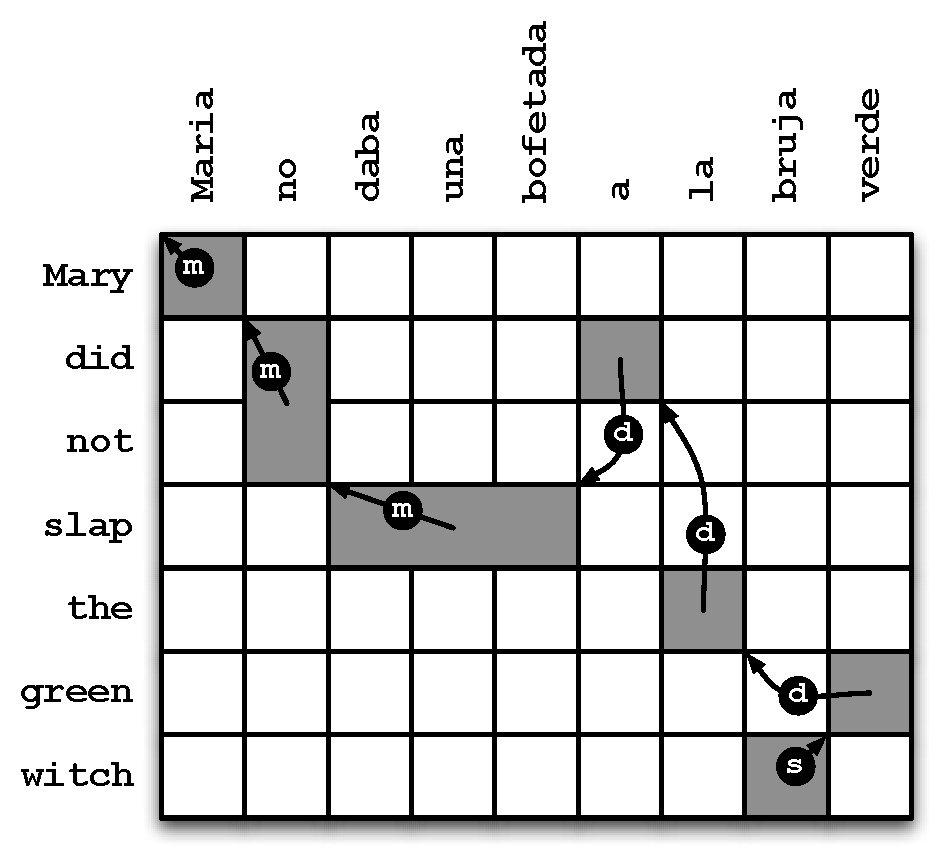
\includegraphics[width=0.8 \linewidth]{../figures/reorderfeats/reorderfeats.pdf}
\caption{The reordering probabilities from the phrase-based models are estimated from bilingual data by calculating how often in the parallel corpus a phrase pair $(f, e)$ is orientated with the preceding phrase pair in the 3 types of orientations (monotone, swapped, and discontinuous). }
\label{fig:reorderfeats} 
\end{center}
%\vskip -0.2in
\end{figure}



\subsection{Bilingual lexicon induction for SMT} \label{sect:bckg:lexind}

{\it Bilingual lexicon induction} describes the class of algorithms that attempt to learn translations from monolingual corpora.   \newcite{Rapp:1995} was the first to propose using non-parallel texts to learn the translations of words.  Using large, unrelated English and German corpora (with 163m and 135m words) and a small German-English bilingual dictionary (with 22k entires), \newcite{Rapp:1999} demonstrated that reasonably accurate translations could be learned for 100 German nouns that were not contained in the seed bilingual dictionary.  His algorithm worked by 
(1) building context vector representing an unknown German word by counting its co-occurrence with all the other words in the German monolingual corpus,
(2) projecting this German vector onto the vector space of English using the seed bilingual dictionary,
(3) calculating the similarity of this sparse projected vector to vectors for English words that were constructed using the  English monolingual corpus, and
(4) outputting the English words with the highest similarity as the most likely translations.

% the context of a given word as a clue to its translation.  The model populates a bilingual lexicon by using a small seed dictionary to project context vectors across two languages and to score their similarity. 
%\newcite{Rapp:1995} was the first to propose using the context of a given word as a clue to its translation.  The model populates a bilingual lexicon by using a small seed dictionary to project context vectors across two languages and to score their similarity. 

A variety of subsequent work has extended the original idea either by exploring different measures of vector similarity \cite{Fung:1998} or by proposing other ways of measuring similarity beyond co-occurence within a context window.  For instance, \newcite{Schafer:2002} demonstrated that word translations tend to co-occur {\it in time} across languages. 
%\newcite{Klementiev:2006b} used this temporal cue to train a phonetic similarity model for associating Named Entities across languages.  
\newcite{Koehn:2002} used similarity  {\it in spelling} as another kind of cue that a pair of words may be translations of one another.
\newcite{Garera2009} defined context vectors using {\it dependency relations} rather than adjacent words.
\newcite{BergsmaVanDurmeIJCAI11} used the {\it visual similarity} of labeled web images to learn translations of nouns.
Additional related work on learning translations from monolingual corpora is discussed in Section \ref{sect:related-work}.

% In this work, we extend these ideas and utilize four independent metrics to score {\em phrasal} translation candidates.  

\begin{figure}[t]
\begin{center}
\vspace{-.5cm}
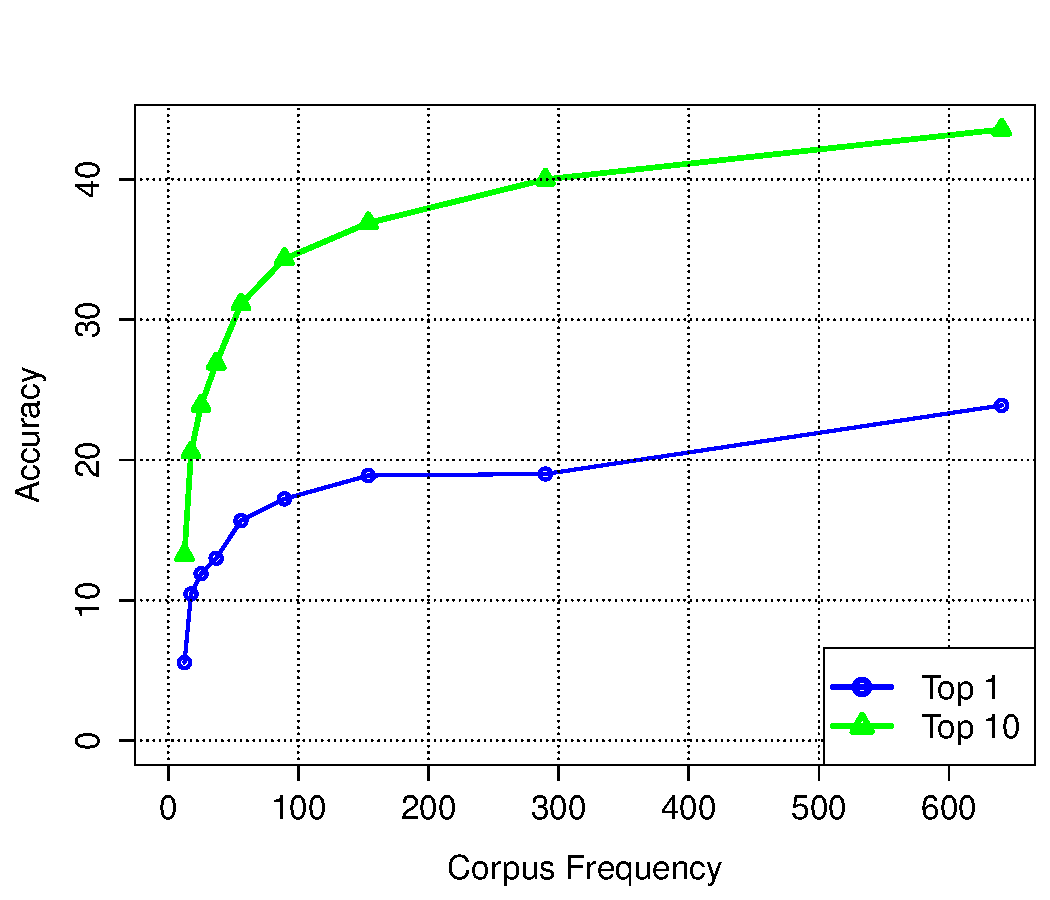
\includegraphics[width=\linewidth]{../figures/lexinductnew/lexinductnew.pdf}
\vspace{-.5cm}
\caption{Accuracy of single-word translations induced using contextual similarity as a function of the source word corpus frequency.  Accuracy is the proportion of the source words with at least one correct (bilingual dictionary) translation in the top 1 and top 10 candidate lists.  }
\label{fig:lexinduct}
\end{center}
\vskip -0.2in
\end{figure}


In this paper, we apply bilingual lexicon induction methods to statistical machine translation.  Given the obvious benefits of not having to rely on scarce bilingual parallel training data, it is surprising that  bilingual lexicon induction has not previously been used for SMT.
There are several open questions that make its applicability to SMT uncertain.  Previous research into bilingual lexicon induction learned translations only for a small number of high frequency words (e.g. 100 nouns in \newcite{Rapp:1995}, 1,000 most frequent words in \newcite{Koehn:2002}, or 2,000 most frequent nouns in \newcite{Haghighi:2008}).  Although previous work reported high translation accuracy, it may be misleading to extrapolate the results to SMT, where it is necessary to translate a much larger set of words and phrases, including many low frequency  items. 

As a preliminary study we plotted the accuracy of translations against the frequency of the source words in the monolingual corpus.  \figref{fig:lexinduct} shows the result for translations induced using contextual similarity (defined in \secref{sect:phrasalfeats}). Unsurprisingly, frequent terms have a substantially better chance of being paired with a correct translation, with words that only occur once having a low chance of being translated accurately.\footnote{For a description of the experimental setup that was used to  produce these translations, see Experiment 8 in Section \ref{sec:results:bitext}.}  This problem is exacerbated when we move to multi-token phrases.  As with phrase translation features estimated from parallel data, longer phrases are more sparse, making similarity scores less reliable than for single words. 

Another impediment (not addressed in this paper) for using lexicon induction for SMT is the number of translations that must be learned.   Learning translations for all words in the source language requires $n^2$ vector comparisons, since each word in source language vocabulary must be compared against the vectors for all words in the target language vocabulary.   The size of the $n^2$ comparisons hugely increases if we compare vectors for multi-word phrases instead of just words. 
%
In this work, we avoid this problem by assuming that a limited set of phrase pairs is given a priori (but without scores).  By limiting ourselves to phrases in a phrase table, we vastly limit the search space of possible translations.  This is an idealization because high quality translations are guaranteed to be present.   However, as our lesion experiments in Section \ref{sect:exp:lesions} show, a phrase table without accurate translation probability estimates is insufficient to produce high quality translations.  We show that lexicon induction methods can be used to replace bilingual estimation of phrase- and lexical-translation probabilities, making a significant step towards SMT without parallel corpora.

%Sparsity is a major concern when scoring MT sized phrase tables, and we propose to deal with in two ways.  First, in \secref{sect:phrasalfeats} we propose to use multiple cues intrinsic to monolingual data as independent evidence when scoring translation candidates.  Second,  in \secref{sect:lexfeats}, we introduce additional similarity estimates less prone to phrasal sparsity issues.

%In \secref{sect:exp:lesions} we show that monolingual features are very informative and reliable in our setting; even when added alongside the feature functions derived from parallel data, they yield substantial BLEU score improvements (over a point in our Spanish-English MT experiments).

%Second, extending the bilingual lexicon induction methods to the induction of multi-word translation pairs greatly increases computational cost. Since each source-target pair must be scored, we would need to compute $|V_{f}| * |V_{e}|$ similarity scores, where $|V_{f}|$ and $|V_{e}|$ are the number of unique items in the source and target vocabularies. When we move from tokens to multi word phrases, $|V|$ grows to the number of unique {\it n}-grams. Exhaustively scoring all phrase pairs up to length three, for example, requires computing scores between the set of unique unigrams, bigrams and trigrams in the source and target languages.  In \secref{sect:extract}, we propose methods to substantially reduce the number of comparisons, while keeping good translation candidates.

%By comparison, \newcite{Rapp:1999} originally evaluated his bilingual lexicon induction only on a collection of 100 manually selected German nouns.  For computational reasons, the number of vector comparisons was reduced by comparing these nouns only against English words with a frequency $\geq100$ in the monolingual corpus.
% Rapp reports that his English monolingual corpus has 657,787 word types after lemmatization, but does not report how many remain after thresholding.
%\newcite{Koehn:2002} used a test set consisting of the 1000 most frequent nouns from a German-English lexicon.  They performed only one million vector comparisons between the 1000 most frequent German nouns and the 1000 most frequent English nouns.
%\newcite{Haghighi:2008} learn translations for only the 2000 most frequent nouns.   \newcite{Garera2009} expand beyond nouns to any part of speech, but still only extract translations of the 1000 most frequent words.

% ------------------------------------------------

\section{Monolingual Parameter Estimation} \label{sect:mono}

We use  bilingual lexicon induction to estimate the parameters of a phrase-based translation model from monolingual data. Instead of scores estimated from bilingual parallel data, we make use of cues present in monolingual data to provide multiple orthogonal estimates of similarity between a pair of phrases. 

%In Sections \ref{sect:phrasalfeats} and \ref{sect:lexfeats}, we introduce two kinds of scores we call {\em phrasal} and {\em lexical similarity} features.  The former score entire phrases, while the latter use word-level alignments between the phrase pairs to calculate lexical scores.  The motivation is analogous to the two kinds of features we reviewed in \secref{sect:bckg:smt}: lexical similarity features are informative for rare phrases that have less reliable phrasal similarity scores because of sparse counts. 

\subsection{Phrasal similarity features} \label{sect:phrasalfeats}



\begin{figure}[t]
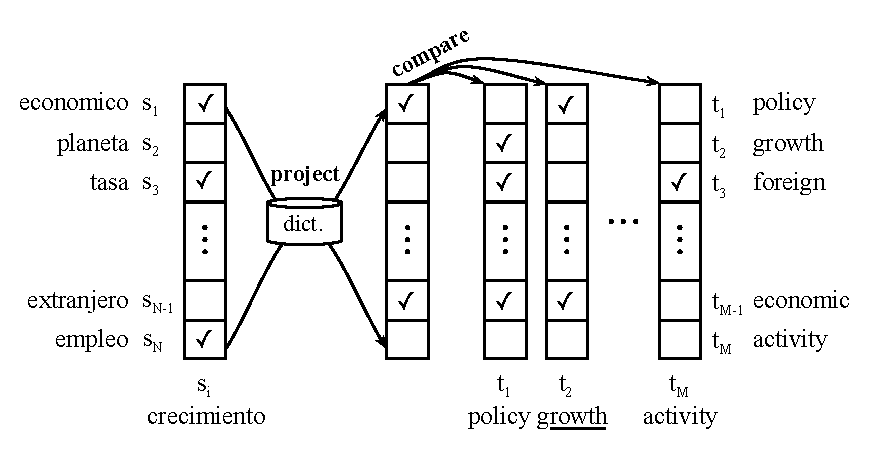
\includegraphics[width=\linewidth]{../figures/contextual/contextual}
\caption{Scoring contextual similarity of \emph{phrases}: first, contextual vectors are projected using a small seed dictionary and then compared with the target language candidates.}
\label{fig:contextual}
\end{figure}


\paraheader{Contextual similarity.}  We extend the vector space approach of \newcite{Rapp:1999} to compute similarity between \emph{phrases} in the source and target languages.  More formally, assume that $(s_{1}, s_{2}, \dots s_{N})$ and $(t_{1}, t_{2}, \dots t_{M})$ are (arbitrarily indexed) source and target vocabularies, respectively.  A source phrase $f$ is represented with an $N$- and target phrase $e$ with an $M$-dimensional vector (see \figref{fig:contextual}).  
The component values of the vector representing a phrase correspond to how often each of the words in that vocabulary appeared within a two word window on either side of the phrase.  These counts are collected using the monolingual corpora. 
After the values have been computed, a contextual vector $f$ is projected onto English vector space using the translations in a seed bilingual dictionary to map the component values into their appropriate positions in an English vector. This sparse projected vector is compared to the vectors representing all English phrases $e$.  Each phrase in a the phrase table is assigned a contextual similarity score $c(f, e)$ based on the similarity between $e$ and the projection of $f$.  

Various means of computing the component values and vector similarity measures have been proposed in literature (e.g. \newcite{Rapp:1999}, \newcite{Fung:1998}).  Following \newcite{Fung:1998}, we compute the value of the $k$-th component of $f$'s contextual vector  as follows: 
\begin{equation*}
w_{k} = n_{f,k} \times (log( {n / n_{k}}) + 1)
\end{equation*}
\noindent where $n_{f,k}$ and $n_{k}$ are the number of times $s_{k}$ appears in the context of $f$ and in the entire corpus, and $n$ is the maximum number of occurrences of any word in the data.  Intuitively, the more frequently $s_{k}$ appears with $f$ and the less common it is in the corpus in general, the higher its component value.  Similarity between two resulting vectors is measured as a cosine of the angle between them.

%\mtodo{Give an example Spanish phrase and the English phrases that it has the highest similarity with}


\begin{figure}[t]
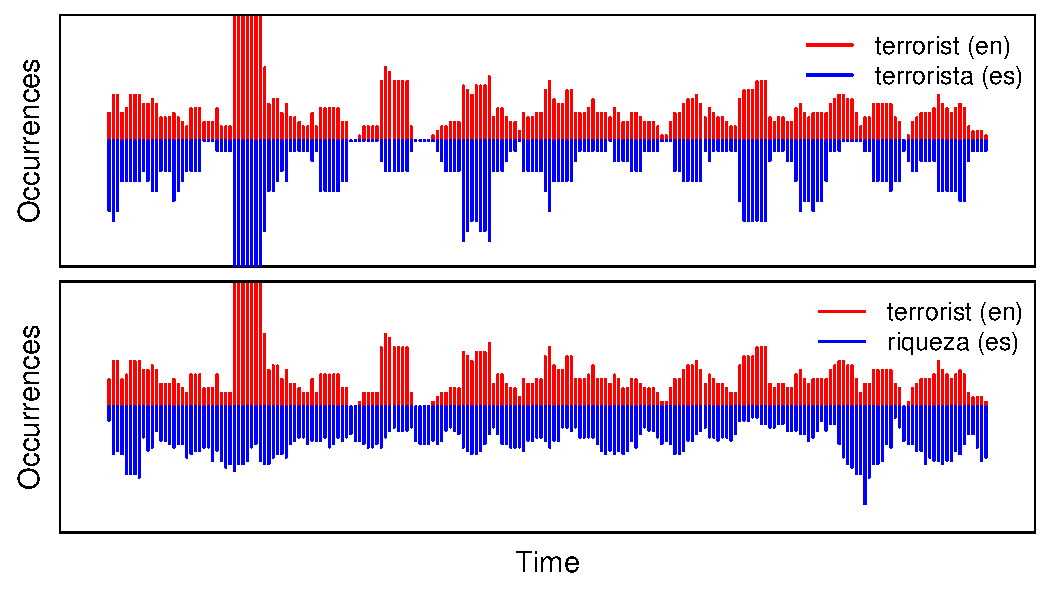
\includegraphics[width= \linewidth]{../figures/temporal/temporal}
\caption{Temporal histograms of the English phrase {\em to terrorists}, its Spanish translation {\em a los terroristas}, and the phrase {\em y riqueza} (and wealth) collected from monolingual texts spanning a 13 year period. While the correct translation has a good temporal match, the non-translation {\em y riqueza} has a distinctly different signature.}
\label{fig:temporal}
\end{figure}




\paraheader{Temporal similarity.} In addition to contextual similarity, phrases in two different languages may be scored in terms of their temporal similarity \cite{alfonseca-ciaramita-hall:2009:EMNLP}.  The intuition is that news stories from different countries will tend to discuss the same world events on the same day.  The frequencies of phrases over time give them a particular signature that will tend to spike on the same dates across languages.  For instance, if the phrase {\it asian tsunami} is used frequently during a particular time span, the number of mentions of the Spanish phrase {\it maremoto asi\'{a}tico} is very likely to increase in the same timeframe. \figref{fig:temporal} illustrates how the temporal distribution of {\it to terrorists} is more similar to the Spanish {\it a los terroristas} than to other Spanish phrases.  We calculate the temporal similarity between a pair of phrases $t(f, e)$ using the method defined by \newcite{Klementiev:2006b}.   A temporal signature for each phrase is generated by sorting the set of (time-stamped) documents in the monolingual corpus into a sequence of equally sized temporal bins and by counting the number of phrase occurrences in each bin.  The our experiments, we set the window size to 1 day, so the size of temporal signatures equals to the number of days spanned by our corpus.  Cosine distance is used to compare the normalized temporal signatures for a pair of phrases  $(f, e)$.

\paraheader{Topic similarity.}\mtodo{Spin this as a new feature! Also: explain it in a little more detail} Phrases and their translations are likely to appear in articles written about the same topic in two languages.  Thus, topic or category information associated with monolingual data can also be used to indicate similarity between a phrase and its candidate translation.  In order to score a pair of phrases, we can collect their topic signatures by counting their occurrences in each topic and then comparing the resulting vectors.  We again use the cosine similarity measure on the normalized topic signatures.  In our experiments, we use interlingual links between wikipedia articles to estimate topic similarity.  We treat each linked article pair as a topic and collect counts for each phrase across all articles in its corresponding language.  Thus, the size of a phrase topic signature is the number of article pairs with interlingual links in Wikipedia, and each component contains the number of times the phrase appears in (the appropriate side of) the corresponding pair.  Our Wikipedia-based topic similarity feature, $w(f, e)$, is similar in spirit to polylingual topic models \cite{Mimno:2009}, but it is scalable to full bilingual lexicon induction.

\vspace{-.1cm}
\subsection{Lexical similarity features}  \label{sect:lexfeats}

In addition to the three phrase similarity features used in our model -- $c(f, e), t(f, e)$ and $w(f, e)$ -- we include four additional {\it lexical similarity features} for each of phrase pair.  The first three lexical features $c_{lex}(f, e), t_{lex}(f, e)$ and $w_{lex}(f, e)$ are the lexical equivalents of the phrase-level {\it contextual, temporal} and {\it wikipedia topic} similarity scores.  They score the similarity of individual words within the phrases.  To compute these lexical similarity features, we average similarity scores over all possible word alignments across the two phrases. 
Because individual words are more frequent than multiword phrases, the accuracy of $c_{lex},  t_{lex}$, and $w_{lex}$  tends to be higher than their phrasal equivalents (this is similar to the effect observed in Figure \ref{fig:lexinduct}). 

\paraheader{Orthographic / phonetic similarity.}  The final lexical similarity feature that we incorporate is $o(f, e)$, which measure the orthographic similarity between words in the translations. 
Etymologically related words often retain similar spelling across languages with the same writing system, and low string edit distance sometimes signals translation equivalency.  
We can also extend this idea to language pairs not sharing the same writing system since many cognates, borrowed words, and names remain phonetically similar.  Transliterations can be generated for tokens in a source phrase (e.g. \newcite{Knight1997}), with $o(f, e)$ now calculating phonetic similarity rather than orthographic.

The three phrasal and four lexical similarity scores are incorporated into the  log linear translation model as feature functions, replacing the bilingually estimated phrase translation probabilities $\phi$ and lexical weighting probabilities $w$.  Our seven similarity scores are not only ones that could be incorporated into the translation model. Various other similarity scores can be computed depending on the available monolingual data and its associated metadata (see, e.g. \newcite{Schafer:2002}).

\vspace{-.1cm}
\subsection{Reordering} \label{sect:order}

\SetAlFnt{\relsize{-1.5}}

\begin{algorithm}[t]

 \SetKwFunction{CollectOccurs}{CollectOccurs}
 \SetKwBlock{Body}{}{}
 \SetCommentSty{text}
 \SetFuncSty{text}

 \hrule \vskip 0.2cm

  \KwIn{Source and target phrases $f$ and $e$,\\
  \hskip 0.85cm Source and target monolingual corpora $\emph{C}_f$ and $\emph{C}_e$,\\
  \hskip 0.85cm Phrase table pairs $\emph{T} = \{(f^{(i)}, e^{(i)})\}_{i=1}^{N}$.}
  \KwOut{Orientation features ($p_m, p_s, p_d$).}
  
  \vskip 0.2cm \hrule \vskip 0.2cm

  $S_f \leftarrow$ sentences containing $f$ in $\emph{C}_f$\;
  $S_e \leftarrow$ sentences containing $e$ in $\emph{C}_e$\;
  
  $(B_f, -, -) \leftarrow \CollectOccurs(f, \cup_{i=1}^{N} f^{(i)}, S_f)$\;
  $(B_e, A_e, D_e) \leftarrow \CollectOccurs(e, \cup_{i=1}^{N} e^{(i)}, S_e)$\;
    
  $c_m = c_s = c_d = 0$\;
  
  \vskip 0.1cm 

  \ForEach{unique $f'$ in $B_f$} {
    \ForEach{translation $e'$ of $f'$ in $\emph{T}$} {

      $c_m = c_m + \#_{B_e}(e')$\; 
       $c_s = c_s + \#_{A_e}(e')$\; 
       $c_d = c_d + \#_{D_e}(e')$\; 
    }
  }
  
  $c \leftarrow c_m + c_s + c_d$;
    
  \Return{$({c_m \over c}, {c_s \over c}, {c_d \over c})$}

  \vskip 0.2cm \hrule \vskip 0.2cm

  \CollectOccurs{$r$, $R$, $S$} \Body{
   $B \leftarrow ()$; $A \leftarrow ()$; $D \leftarrow ()$\;

    \ForEach{sentence $s \in S$} {
      \ForEach{occurrence of phrase $r$ in $s$} {
        $B \leftarrow B$ + $($longest preceding $r$ and in $R)$\;
        $A \leftarrow A$ + $($longest following $r$ and in $R)$\;
        $D \leftarrow D$ + $($longest discontinuous w/ $r$ and in $R)$\;
      }
    }
    
    \Return{($B$, $A$, $D$)}\;
  }
  
  \vskip 0.2cm \hrule \vskip 0.2cm

  \caption{Algorithm for estimating reordering probabilities from monolingual data.} \label{fig:algoreorder}
  \vskip -0.2in
\end{algorithm}


\begin{figure}[t]
%\vskip 0.1in
\begin{center}
\vspace{-.5cm}
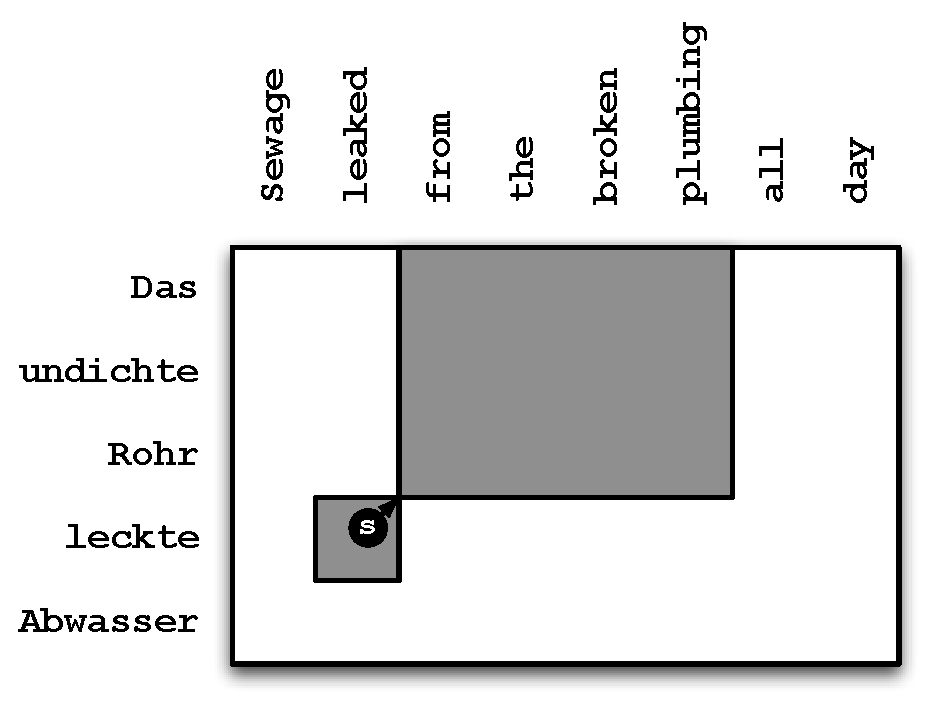
\includegraphics[width=0.8 \linewidth]{../figures/monoreord/monoreord.pdf}
\caption{Collecting phrase orientation statistics for a en-de phrase pair (\emq{profile}, \emq{Profils}) from non-parallel sentences (the German sentence translates as  \emq{Creating a Facebook profile is easy}). The longest preceding phrase \emq{Facebook} in source, has a phrase table translation \emq{in Facebook} appearing after the target phrase.}
\label{fig:monoreord}
\end{center}
\vskip -0.2in
\end{figure}

The remaining component of phrase-based SMT model is the reordering model. We introduce a novel algorithm for estimating $p_o(\textnormal{orientation}|f,e)$ from two monolingual corpora instead a bitext.

%\todo{ccb - rewrite the first paragraph}
Figure \ref{fig:reorderfeats} illustrates how the phrase pair orientation statistics are estimated in the standard phrase-based SMT pipeline.  For a phrase pair like ($f =$ \emq{Profils}, $e =$ \emq{profile}), we count its orientation with the previously translated phrase pair ($f' =$ \emq{in Facebook}, $e' =$ \emq{Facebook}) across all translated sentence pairs in the bitext.  

In our pipeline we do not have translated sentence pairs.  Instead, we look for monolingual sentences in the source corpus which contain the source phrase that we are interested in, like $f =$ \emq{Profils}, and at least one other phrase that we have a translation for, like $f' =$ \emq{in Facebook}.  We then look for all target language sentences in the target monolingual corpus that contain the translation of $f$ (here $e =$ \emq{profile}) and any translation of $f'$.  \figref{fig:monoreord} illustrates that it is possible to find evidence for $p_o(\textnormal{swapped}| \it{ Profils},\it{ profile})$, even from the non-parallel, non-translated sentences drawn from two independent monolingual corpora.  By looking for foreign sentences containing pairs of adjacent foreign phrases $(f, f')$ and English sentences containing their corresponding translations $(e, e')$, we are able to increment orientation counts for $(f, e)$ by looking at whether $e$ and $e'$ are adjacent, swapped, or discontinuous, much in the same way as in Fig.~\ref{fig:reorderfeats}.

One subtly of our method is that 
%In the phrase-based SMT pipeline, phrase pair orientation statistics are collected using word alignments.  We keep a similar reordering model formulation but infer its parameters from monolingual data instead.  The orientation information for a phrase pair ($f$, $e$) is collected from source and target sentences containing ($f$, $e$) as well as other phrase pairs.  Suppose one such sentence pair contains another pair of phrases ($f'$, $e'$), and that $f'$ is immediately adjacent to $f$.  The idea is to check whether $e'$ stays in the same order with $e$, swaps, or becomes discontinuous in the target sentence. Consider the simple example in \figref{fig:monoreord}: the phrase pair is ($f =$ \emq{profile}, $e =$ \emq{Profils}), and a given pair of non-parallel sentences also contains a phrase table entry ($f' =$ \emq{Facebook}, $e' =$ \emq{in Facebook}).  In this example, the phrase $f'$ preceding $f$ in the source sentence swaps order with $e$ in the target.  When we collect these counts over large monolingual corpora, we expect the swap, monotone, and discontinuous counts to provide good estimates for the orientation features (\figref{fig:algoreorder}).
%Note that multiple phrases may immediately precede $f$ and appear in the phrase table; however, we only use the longest of them to collect reordering counts.  
shorter and more frequent phrases (e.g. punctuation) are more likely to appear in multiple orientations with a given phrase, and therefore provide poor evidence of re-ordering.  Therefore, we (a) collect the longest contextual phrases (which also appear in the phrase table) for reordering feature estimation, and (b) prune the set of sentences so that we only keep a small set of least frequent contextual phrases (this has the effect of dropping many function words and punctuation marks and and relying more heavily on multi-word content phrases to estimate the reordering).\footnote{The pruning step has an additional benefit of minimizing the memory needed for orientation feature estimations.}


% ------------------------------------------------

\begin{table*}[t]
\begin{tabular}{ll}

\begin{tabular}{lrrr}
\multicolumn{4}{c}{Monolingual training corpora}\\
\hline
 & Europarl & Gigaword & Wikipedia\\
\hline
% date range & 4/15/96-10/22/09	& 5/12/94-12/31/08\\
date range & 4/96-10/09 & 5/94-12/08	& n/a\\
uniq shared dates & 829 & 5,249 & n/a \\
% number of Spanish and English articles is overestimated;
% that's the full set rather than just the ones in the paired dates that we used.
Spanish articles & n/a & 3,727,954 & 59,463 \\
English articles& n/a & 4,862,876 & 59,463 \\
Spanish lines	& 1,307,339 & 22,862,835 & 2,598,269\\
English lines	& 1,307,339 & 67,341,030 & 3,630,041\\
Spanish words & 28,248,930 & 774,813,847 & 39,738,084 \\
English words & 27,335,006 & 1,827,065,374 & 61,656,646\\
%
\end{tabular}
&

\begin{tabular}{lr}
\multicolumn{2}{c}{Spanish-English phrase table}\\
\hline
Phrase pairs & 3,093,228\\
Spanish phrases & 89,386\\
English phrases & 926,138\\
\hline
Spanish unigrams & 13,216\\
\rowcolor{lightgray} Avg \# translations & 98.7\\
Spanish bigrams & 41,426\\
\rowcolor{lightgray} Avg \# translations & 31.9\\
Spanish trigrams & 34,744\\
\rowcolor{lightgray} Avg \# translations & 13.5\\
\end{tabular}
\\

\end{tabular}

\caption{Statistics about the monolingual training data and the phrase table that was used in all of the experiments. 
% The dates were paired, so dates that had articles in one language but not the other were discarded.
}\label{table:training-data+phrase-table}
\end{table*}
% ------------------------------------------------

Our algorithm for learning the reordering parameters is given on \figref{fig:algoreorder}.  The algorithm estimates a probability distribution over monotone, swap, and discontinuous orientations ($p_m$, $p_s$, $p_d$) for a phrase pair ($f, e$) from two monolingual corpora $C_f$ and $C_e$.  It begins by calling {\tt \small CollectOccurs} to collect the longest matching phrase table phrases preceding $f$ in source monolingual data ($B_f$), as well as preceding ($B_e$), following ($A_e$), and discontinuous ($D_e$) phrases with $e$ in the target language data.  For each unique phrase $f'$ preceding $f$, translations are then looked up in the phrase table $\emph{T}$.  Next, we count\footnote{$\#_{L}(x)$ returns the count of object x in list L.} how many translations $e'$ of $'$ appeared before, after or were discontinuous with $e$ in the target language data.  Finally, the counts are normalized and returned.  %The algorithm requires a single pass through the data to collect contextual phrases for the entire phrase table and its running time is quadratic in the size of the table.\mtodo{Check}
%
These normalized counts are the values we use as estimates of $p_o(\textnormal{orientation}|f,e)$. %This allows us to estimate all of the parameters of the phrase-based translation model from monolingual corpora.


%\subsection{Extracting a phrase table without a bitext}  \label{sect:extract}
%Where do we get the phrase table if we cannot extract it from word-aligned sentence pairs? We propose three methods: (1) We implement several ways to prune the space of phrase pair comparisons, which allow us to extend past efforts in bilingual lexicon induction from monolingual corpora to multi-word phrases. (2) We build a table of phrase pair translations by composing phrases using an existing bilingual seed dictionary. (3) We identify \emph {unigrams} in our development and test sets that are OOV in our existing bilingual dictionary and then use a bilingual lexicon induction framework to induce new translations for each. In Section \ref{sect:exp:pt} we perform end-to-end MT experiments to test the quality of these phrase tables both individually and combined.

%\paraheader{Phrase table induction.} As we argued in \secref{sect:bckg:lexind}, we cannot na\"{i}vely extend translation lexicon induction techniques to induce phrasal translations because the search space is too large. We must aggressively prune it.   Specifically, we compare phrases in the same frequency bands \cite{Uszkoreit:2010}, disallow unigram-trigram pairs, and prune very low frequency target phrases. We also use a filter that requires stemmed versions of each phrase-pair to contain at least one (source unigrams and bigrams) or two (source trigrams) word-pairs from a stemmed version of our bilingual dictionary.\footnote{Our stemmer truncates words to a max. of six characters.} %\todo{Alt wording:} We compare  each source side phrase only to target side phrases that occur in the same frequency band (according to the frequencies in two monolingual corpora). Of those target side phrases, we keep only the ones with at least one \mtodo{discuss dictionary parameters} word translating into a word in the source side phrase. 

%To determine whether our pruning parameters are reasonable, we evaluate what percent of the items from a bilingually induced phrase table are retained.  Rather than consider all items from the phrase table (since many of them are bad), we consider only those phrase-pairs that are used by the decoder to translate a test set.\footnote{We use the Moses decoder's trace function to find the set of phrases it used in decoding our test set.} We compare our filtered phrase tables to this set of phrase translation rules and attempt to maintain as many of them as possible, while pruning the set of phrase pairs down to a manageable size. Table \ref{table:prune} shows results using the enumerated heuristics both with the dictionary filter (``Freq+Dict'') and without (``Freq Filter'').

%\paraheader{Dictionary-based phrase table.} We build a second phrase table by enumerating all combinations and permutations of up to three source word dictionary translations \cite{garera08a}. %CUT FOR SPACE Our Spanish--English dictionary has entries for 49,795 source tokens and the resulting phrase table has a large amount of overlap with the decoder table, as shown in Table \ref{table:prune} (``Dict combs''). 
%CUT FOR SPACE: However, for the case of low-resource languages, dictionaries, in the cases that they even exist, are not as complete. We expect the performance of our dictionary-based phrase table to be an upper bound for the performance of an induced-dictionary-composed table for truly low-resource languages.

%\paraheader{Induced lexical translations.} We use a bilingual lexical induction framework that compares context, time, and edit distance source and target word vectors to build a table of candidate translations for the word types (approximately 10,000 for Spanish) in our development and test sets that do not have entries in our bilingual dictionary. In Section \ref{sect:exp:pt} we use this relatively small set of unigram translation pairs to supplement the above tables.
%approximately 3k for Urdu: took out because PT experiments section doesn't have Urdu results

%Our baseline phrase table is generated using a bilingual dictionary. For each Urdu test set phrase up to length three, we generated English phrases from all combinations of dictionary translations and all possible reorderings. For the baseline and our pruning methods, the number of filtered phrase pairs and the percent of phrases used by the Moses decoder not pruned away are given in Table \ref{table:prune}.  

%\begin{table}
%\small
%\begin{center}
%\begin{tabular}{|c|c|c|c|c|}
%\hline
%Pruning 	& Phrase	& Search & 	Findable 	& Findable \\
%filters	& Pairs	&  Space & Types 	&  Tokens \\
%\hline
%\hline
%\multicolumn{5}{|l|}{Spanish} \\
%\hline
%Unpruned & 1.0 T & 100\% & 100\% & 100\% \\
%Dict combs. & 76 M & $<$.01\% & 32\% & 42\% \\
%Freq Filter &  6.2 B & 0.6\% & 54\% & 66\% \\
%Freq + Dict & 324 M & $<$.04\% & 44\% & 54\% \\
%\hline
%\hline
%\multicolumn{5}{|l|}{Urdu} \\
%\hline
%Unpruned & 913 B & 100\% & 100\% & 100\% \\
%Dict combs. & 54 M & $<$.01\% & 15\% & 25\% \\
%Freq Filter & 1.5 B & 0.2\% & 49\% & 62\% \\
%Freq + Dict & 87 M & $<$.01\% & 26\% & 35\% \\
%\hline
%\end{tabular}
%\caption{Tradeoff between pruning the phrase pair search space and accuracy of the final set. Findable types and tokens refer to the percent of phrase types and tokens used by Moses to decode a test set that are not pruned away. The phrase pair count is over phrases in a source side MT dev/test set (Spanish: 2525 sentences, Urdu: 1864 sentences) and in a given target side monolingual corpus (Spanish: English side of Europarl training data, Urdu: English web crawls). The max phrase length is three.}\label{table:prune}
%\end{center}
%\end{table}


%Our baseline phrase table is generated using a bilingual dictionary. For each Urdu test set phrase up to length three, we generated English phrases from all combinations of dictionary translations and all possible reorderings. For the baseline and our pruning methods, the number of filtered phrase pairs and the percent of phrases used by the Moses decoder not pruned away are given in Table \ref{table:prune}.  


%Second round of pruning: after monolingual feature extraction, before re-ordering estimation. \todo{Needs to be discussed after explanation of those methods?}

\section{Experimental Setup} \label{sect:expsetup}

We use the Spanish-English language pair to test our method for estimating the parameters of an SMT system from monolingual corpora.  This allows us to compare our method against the normal bilingual training procedure.  We expect bilingual training to result in higher translation quality, because it is a more direct method for learning translation probabilities.  We systematically remove different parameters from the standard phrase-based model, and then replace them with our monolingual equivalents.  Our goal is to recover as much of the loss as possible for each of the deleted bilingual components. 

The standard phrase-based model that we use as our top-line is the Moses system \cite{Moses} trained over the full Europarl v5 parallel corpus \cite{Koehn:2005}.   With the exception of maximum phrase length (set to 3 in our experiments), default values were used for all of the parameters.  All experiments use a trigram language model trained on the English half of the Europarl corpus using SRILM with Kneser-Ney smoothing. 
To tune feature weights in minimum error rate training, we use a development bitext with 2,553 sentence pairs.  We use the development and test data distributed in WMT shared task \cite{callisonburch-EtAl:2010:WMT}.\footnote{Specifcially, {\em news-test2008} plus {\em news-syscomb2009} for dev and {\em newstest2009} for test.}   The test set is translated newswire articles consisting of 2,525 single-reference sentence pairs.   MERT was re-run for every experiment. 


\begin{figure*}[t]
%\vskip 0.1in
\begin{center}
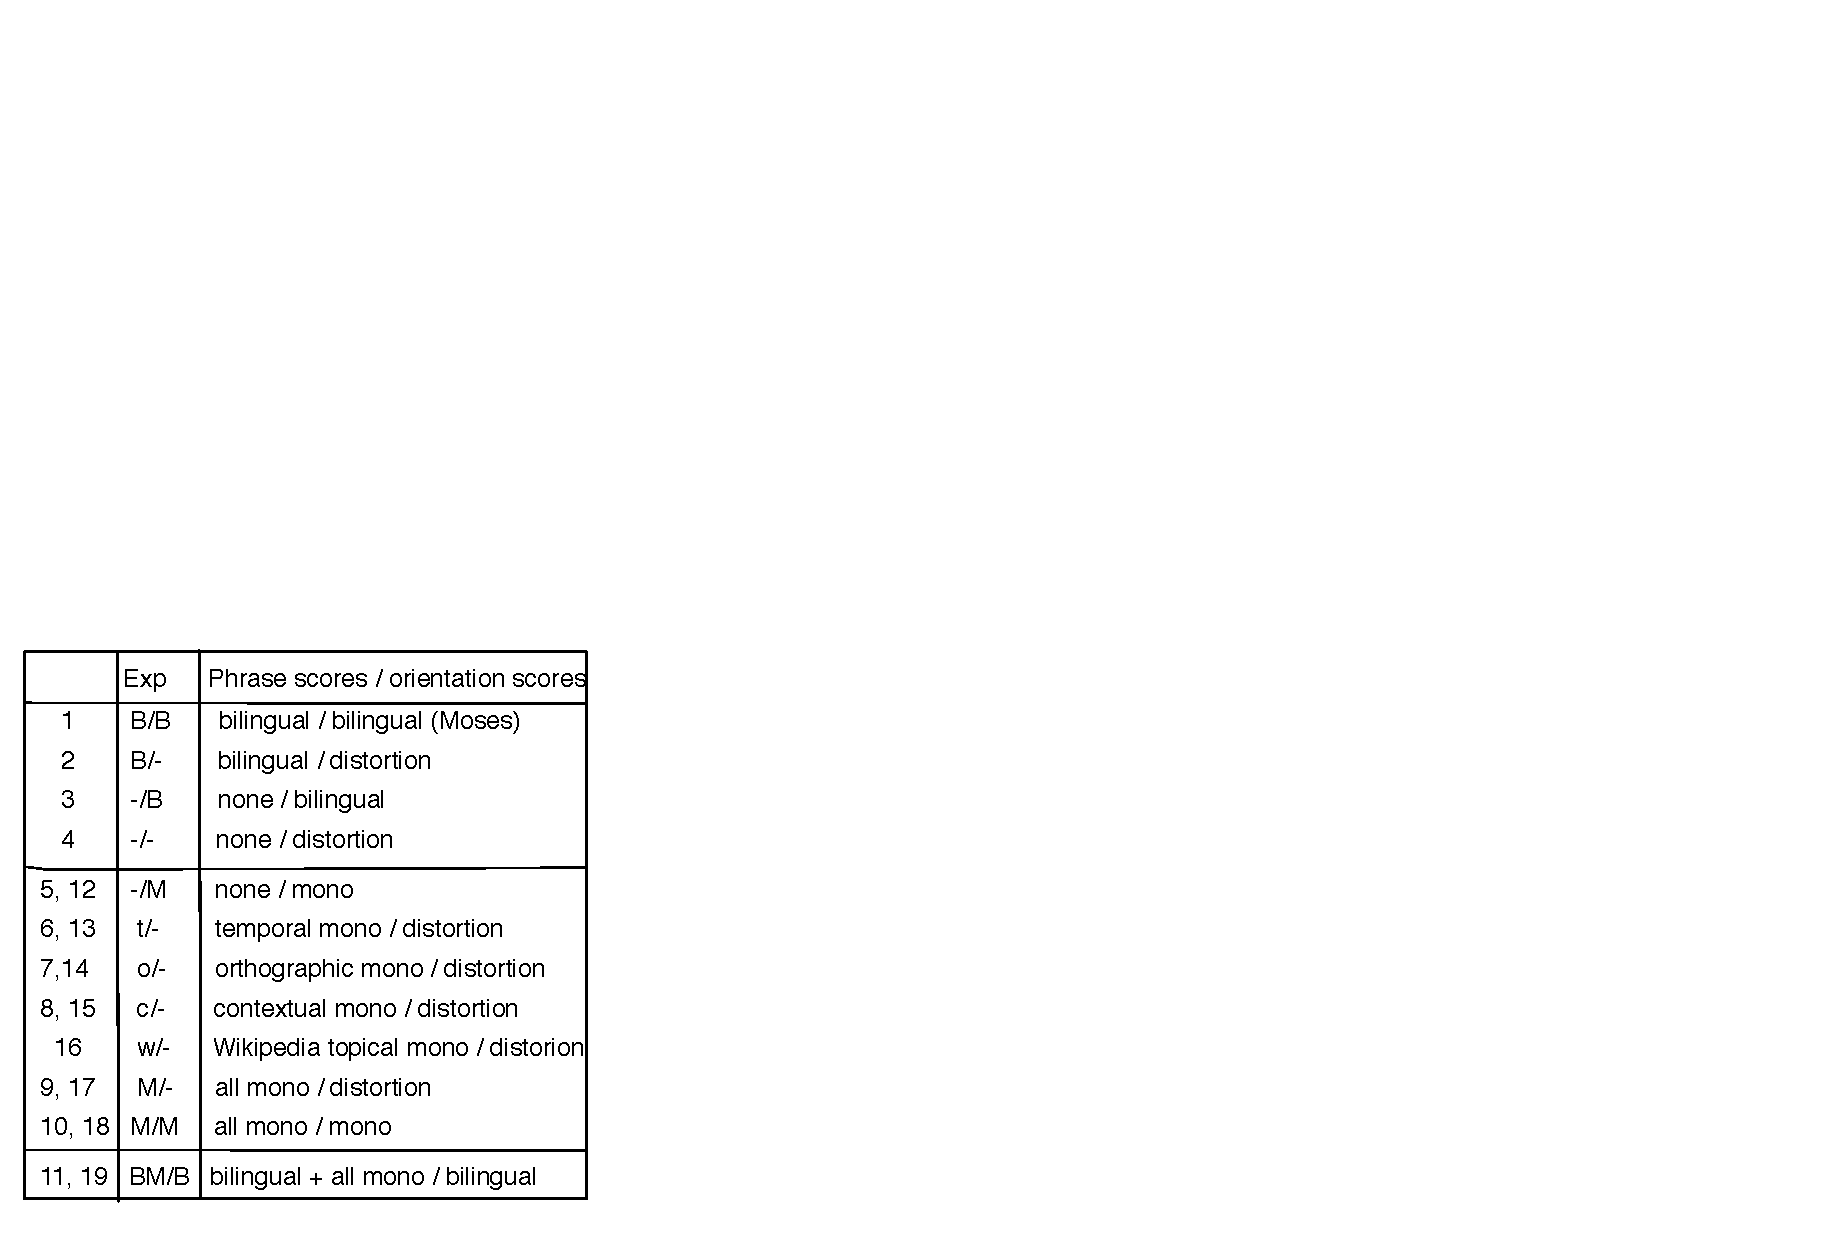
\includegraphics[width=.27\linewidth]{../figures/legend.pdf}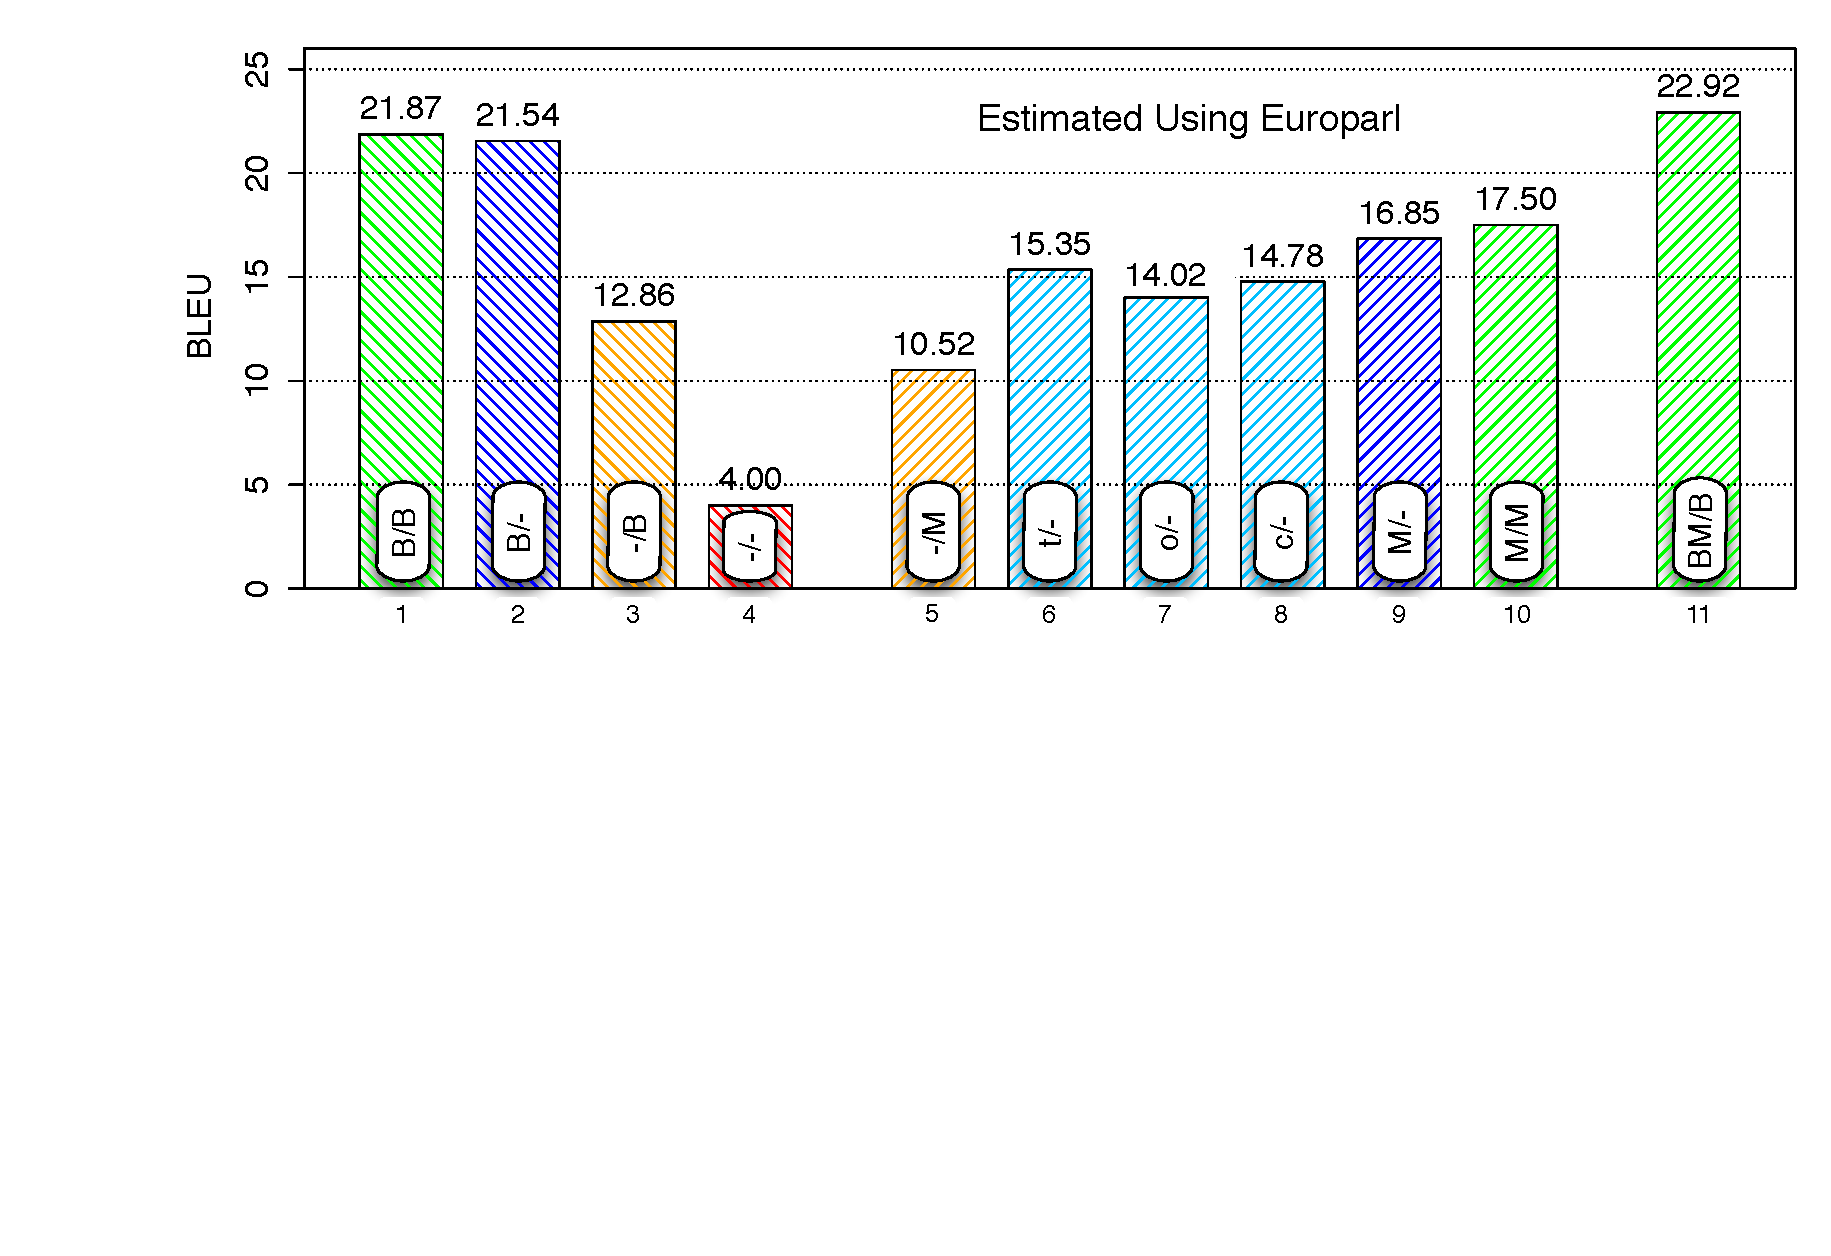
\includegraphics[width=.73\linewidth]{../figures/europarl.pdf}
\caption{Contributions of individual features to overall system performance in Spanish-English experiments derived from parallel texts (experiments 1-4), their monolingual equivalents derived from Europarl data (experiments 5-10)}
\label{fig:lesionreplacement}
\end{center}
\vskip -0.2in
\end{figure*}

We estimate the parameters of our model from two sets of monolingual data, given in Table \ref{table:training-data+phrase-table}:
\begin{itemize}
\item First, we treat the two sides of the Europarl parallel corpus as independent, monolingual corpora.   \newcite{Haghighi:2008} also used this method to show how well translations could be learned from monolingual corpora under ideal conditions, where the contextual and temporal distribution of words in the two monolingual corpora are practically identical.   
\item Next, we estimate the features from truly monolingual corpora.  To estimate the {\it contextual} and {\it temporal} similarity features, we use the Spanish and English Gigaword corpora.\footnote{We use the
%Agence France-Presse (afp), Associated Press Worldstream (apw), and Xinhua News Agency (xin)
afp, apw and xin sections of the corpora.}
These corpora are substantially larger than the Europarl corpora, providing 27x as much Spanish and 67x as much English for contextual similarity, and 6x as many paired dates for temporal similarity. 
%Using real monolingual corpora also allows us 
 {\it Topical} similarity is estimated using Spanish and English Wikipedia articles that are paired with inter-language links.
\end{itemize}
To project context vectors for Spanish to English, we use are a bilingual dictionary containing entries for 49,795 Spanish words.\footnote{End-to-end translation quality is robust to substantially reducing dictionary size; results omitted due to space constraints.}  The context vectors for words and phrases collect co-occurrence counts using a two-word window on either side.

The title of our paper uses the word {\it towards}, because we assume that an inventory of phrase pairs is given. 
Future work shall explore inducing the phrase table itself from monolingual texts.  
Across all of our experiments, we use the phrase table that bilingual model learned from the Europarl parallel corpus.  We keep its phrase pairs, but we drop all of its scores.  Table \ref{table:training-data+phrase-table} gives details of the phrase pairs.  For our experiments, we estimated similarity scores and re-ordering probabilities for more than 3 million phrase pairs.  The set of possible translations were constrained for each source phrase, and therefore were likely to contain good translations.  However, the average number of possible translations was high (ranging from nearly 100 translations for each unigram to 14 for each trigram).  These contain a lot of noise, and result in inferior end-to-end translation quality without good estimates of their translation quality, as the experiments in Section \ref{sect:exp:lesions} will show.

\paraheader{Software.} Because many details of our estimation procedures must be omitted for space, we distribute our full set of code, along with scripts for running our experiments, and output translations.  These may be downed from  \url{url}. \todo{Add  dropbox URL}.





\section{Experimental Results} \label{sect:results}

\todo{ccb - rewrite this section}

We begin by removing each of the standard bilingually estimated features from the SMT model in order to understand their relative contributions to the performance of the end-to-end system (\secref{sect:exp:lesions}). Then, in \secref{sec:results:bitext}, we replace them with monolingual features estimated using the Europarl training corpus but treating each side as an independent, monolingual corpus (i.e., throwing away sentence alignments). In \secref{sec:results:mono}, we estimate the features using truly monolingual corpora.  Finally, in \secref {sec:results:aug} we show substantial improvements to the standard Moses baseline, when its standard features are augmented with the monolingual features we introduced.

\subsection{Lesion experiments (Experiments 1-4)}\label{sect:exp:lesions}
%\paragraph{Lesion experiments (Experiments 1-4)}



We begin with a series of experiments where we remove individual features derived from an aligned bitext in order to get a sense of their relative contributions to the overall system performance on the English-Spanish language pair (see \figref{fig:lesionreplacement}). When both phrase and orientation features are derived from word alignments ({\bf B/B}, the standard features functions defined in \secref{sect:bckg:smt}), the system reaches 21.87 BLEU.  Next we replace orientation features with random values ({\bf B/--}) and drop phrase features ({\bf --/B}).  While phrase table features account for a substantial performance difference (9 BLEU points), dropping orientation features affects the system score relatively little.  This is not surprising, since the word order is generally preserved in Spanish to English translations.  Finally, both dropping phrase scores and replacing orientation features with random values ({\bf --/--}) results in 5.5 BLEU, a 16.4 point drop.  
%This is similar to the only prior art on end-to-end MT without parallel data \cite{Carbonell2006}, which scores translation with a language model alone.

\subsection{Adding equivalent monolingual features estimated using the {\em bitext} (Experiments 5-10)}\label{sec:results:bitext}

Next, we replace the feature functions with their monolingual equivalents estimated using the two sides of the bitext, hoping to regain much of the 16.4 BLEU point loss that resulted from dropping all features.  Adding orientation features estimated from monolingual data alone ({\bf --/M})  recovers 5 BLEU points. The  temporal, orthographic, and contextual monolingual features ({\bf t/--}, {\bf o/--}, and {\bf c/--}) are informative on their own and provide independent evidence for phrase similarity.  Together ({\bf M/--}), they recover over 11 BLEU points.
%Adding phrasal monolingual scores ({\bf P/--}) and lexical monolingual scores ({\bf L/--}) separately recover 8.8 and 10.8 BLEU points, respectively, and 11.3 points together. 
Like the standard translation features estimated from the bitext, our monolingual features contribute more to performance than the reordering feature. Supplementing the stripped phrase table with all of our monolingually estimated features ({\bf M/M}) yields an even higher gain of {\bf 12.0 BLEU} points. %, or {\bf over 80\% of the BLEU score} loss that occurred when we dropped all features from the phrase table. 
Our monolingual features successfully recover much of the information contained in the features derived from bitext.  %Note that the achieved score is equivalent to a standard bilingually estimated system trained on a parallel corpus of roughly 500,000 \todo{is this still the same?} words (learning curve is omitted due to space constraints).
However, here we use monolingual corpora which we know to have very similar phrasal and temporal distributions. In the next section, we drop this idealization.

\subsection{Adding equivalent monolingual features estimated using {\em truly monolingual} corpora (Experiments 12-18)}\label{sec:results:mono}

We now show a similar set of experiments as in the previous section, but this time we estimate all of our features from truly monolingual corpora.
%Instead of treating two sides of the parallel corpus as independent, monolingual corpora, we estimate our features using truly monolingual corpora. 
%As explained in \secref{sect:expsetup}, we estimate contextual and temporal features using subsets of the Spanish and English Gigaword corpora, and we estimate an additional contextual feature, the topical feature, and reordering features using a sample of Spanish and English Wikipedia pages. 
Adding orientation features alone ({\bf --/M}) recovers 4.7 BLEU points, about 0.3 less than adding orientation features estimated using the bitext. Experiments 13-16 show how each monolingually estimated feature impacts MT performance. Each feature is independently capable of recovering at least 7.5 BLEU points above the featureless table. The topical feature is the most independently informative and alone recovers over 11 BLEU points. Together, the four monolingually estimated features ({\bf M/-}) recover over 12.5 points and result in a BLEU score of 18.06. Also using our monolingually estimated reordering feature ({\bf M/M}) yields a total gain of {\bf 13.3 BLEU} points, or {\bf over 81\%} of the BLEU point loss that occurred when we dropped all features from the phrase table.  This result is roughly equivalent to training the standard system on about 60,000 lines of bitext (see \figref{fig:mtlearn}).


\begin{figure}[t]
%\vskip 0.1in
\begin{center}
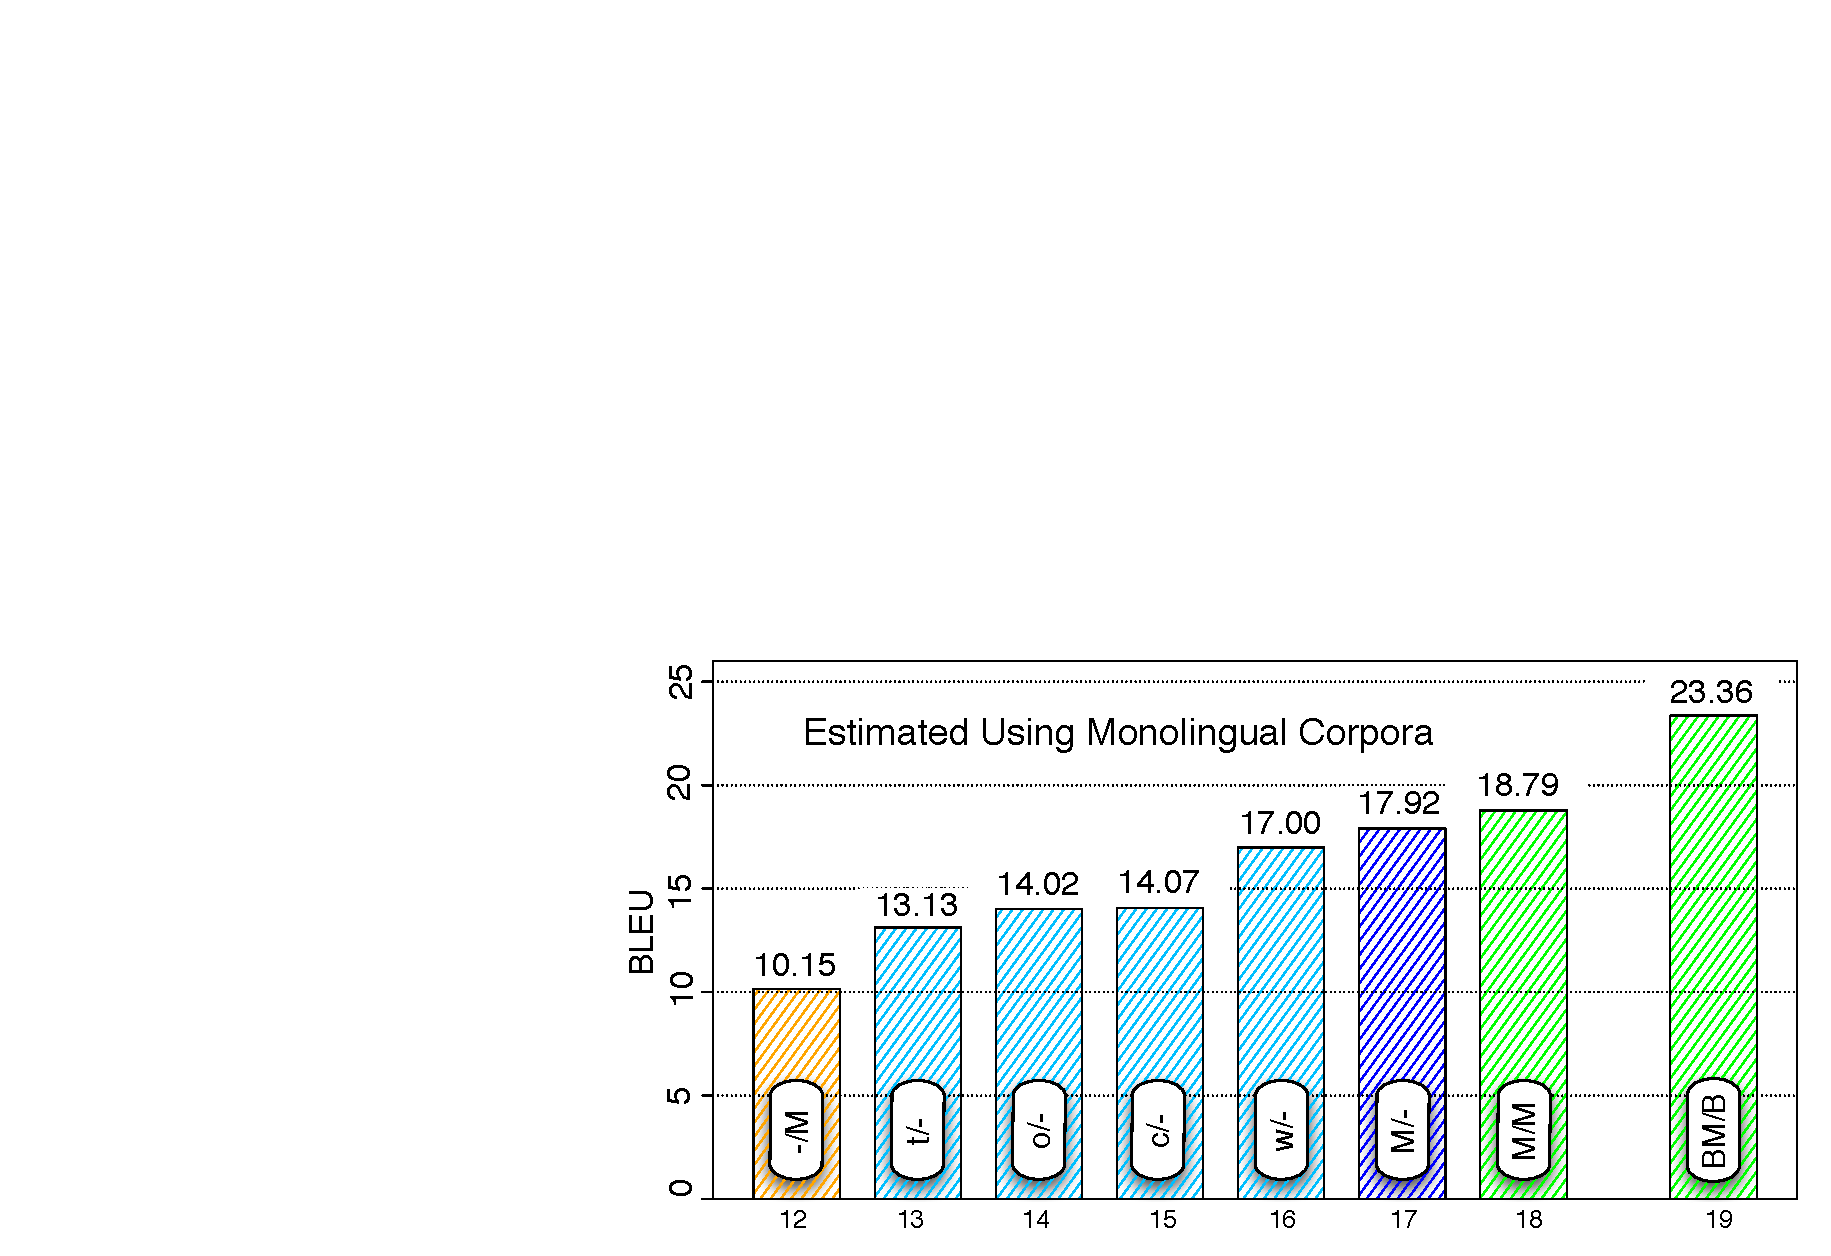
\includegraphics[width=\linewidth]{../figures/monolingual.pdf}
\caption{monolingual equivalents derived from truly monolingual corpora (experiments 12-18).  Over 80\% of lost performance can be recovered with monolingual features estimated using monolingual corpora alone.  Moreover, when added alongside the features derived from parallel data (experiments 11, 19), monolingual features account for for over 1 BLEU point gain (experiment 10).}
\label{fig:lesionreplacement}
\end{center}
\vskip -0.2in
\end{figure}


\begin{figure}[t]
%\vskip 0.1in
\begin{center}
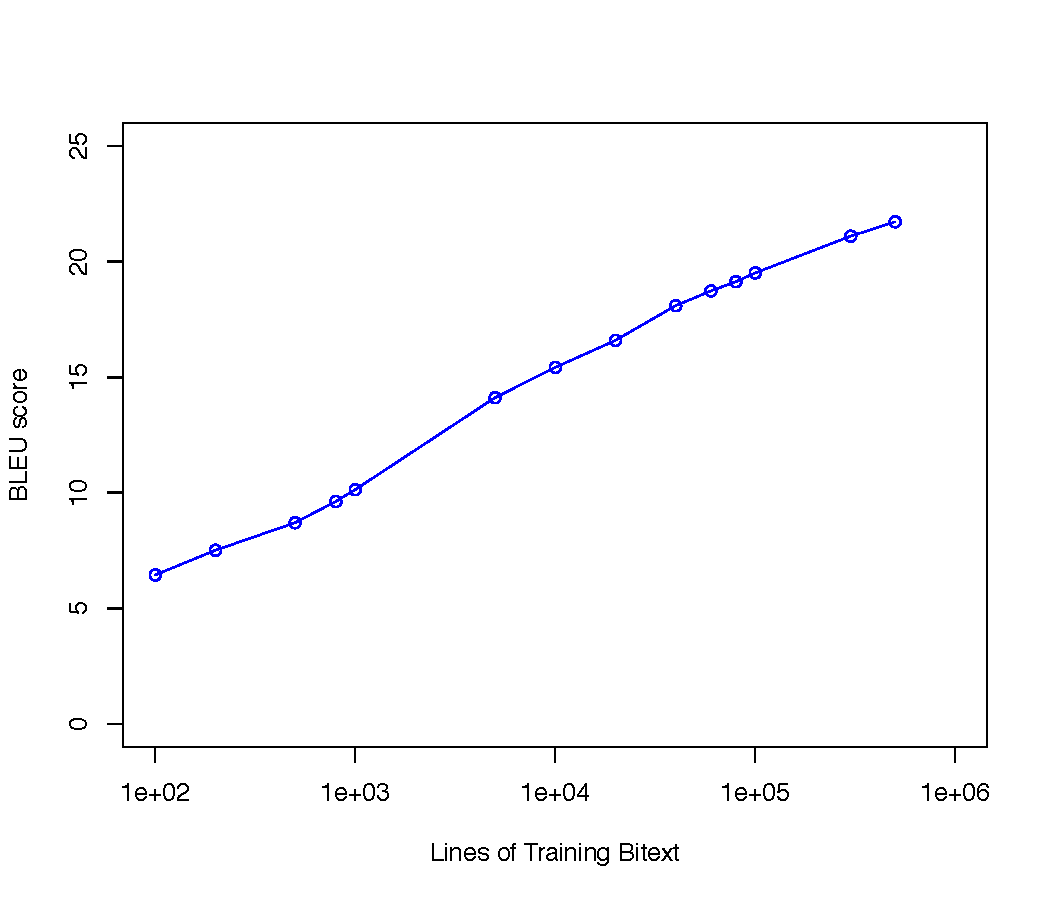
\includegraphics[width=\linewidth]{../figures/mtlearning/esenlearning.pdf}
\caption{Performance of the Moses pipeline ({\bf B/B}) vs. the amount of Spanish-English Europarl training data.}
\label{fig:mtlearn}
\end{center}
\vskip -0.2in
\end{figure}

%However, the phrasal and lexical scores are {\em better} than those estimated using the Europarl bitext; adding them to the stripped phrase table further increases the BLEU score by 1.2 and 0.5 points, respectively, and 1.3 together, {\em beyond} the scores achieved when adding the features estimated using the bitext. This additional gain is likely due to the fact that our monolingual corpora are large relative to the bitext and that we are able to capture a strong orthogonal topical similarity signal. Supplementing the stripped phrase table with all of our features estimated from truly monolingual corpora ({\bf PL/M}) yields a total gain of {\bf 13.3 BLEU} points, or {\bf over 80\% of the BLEU score} loss that occurred when we dropped all features from the phrase table. Note that the achieved score is equivalent to a standard bilingually estimated system trained on a parallel corpus of roughly 500,000 \todo{is this still the same?} words (learning curve is omitted due to space constraints).

\subsection{Augmenting standard features with monolingual features (Experiment 11, 19)} \label{sec:results:aug}
Finally, we perform an additional experiment to determine whether there is any information estimated in monolingual scores that is not captured by the standard feature set derived from the bitext. Indeed, we see a 1.0 BLEU point increase when we supplement the original phrase table with the monolingual phrasal and lexical features estimated using the bitext and {\bf 1.5} BLEU point increase using those estimated from our truly monolingual corpora ({\bf BPL/B}). %Therefore, our monolingually estimated scores capture some novel information not contained in the standard feature set. 

% ------------------------------------------------
\section{Related Work} \label{sect:related-work}

Recent work on lexical induction includes \newcite{Haghighi:2008} who made use of contextual and orthographic clues to learn a generative model from monolingual texts and a seed lexicon.  \newcite{Mimno:2009}  proposed a polylingual topic model and matched high probability words in each topic across languages.  While effective for a small number of topics, it is unlikely to scale well to large multilingual dictionaries. \newcite{BergKirkpatrick2011} learn a correspondence between the alphabets of two languages for cognate identification, which will not generalize to general etymologically unrelated translations. 

%\todop{Chris}{Additional reference pointed out by reviewers worth including?}
\newcite{Carbonell2006} described a data-driven machine translation system that used no parallel text. It produced translation lattices using a bilingual dictionary and scored them using an n-gram language model.  This method is similar to our baseline which eliminates the translation probabilities from a phrase-table, and scores the output only with an n-gram language model.  

We examine scenarios where large bilingual parallel corpora are not available.  A variety of past research has focused on overcoming this bottleneck by mining parallel or comparable corpora from the web \cite{Munteanu:2006,Schwenk2008,Rauf2009,Smith2010,Uszkoreit:2010}.  Methods for acquiring bitexts are complimentary but orthogonal to our research goals.  We focus on the ``no bitext'' condition, but a logical follow-on would be to bootstrap from a small bitext.

\todo{Update with citations: \newcite{Lambert2011}, \newcite{Chen2008}, \newcite{Foster2007}. See comments in .tex.  Also \newcite{ravi-knight:2011:ACL-HLT}, and \newcite{daumeiii-jagarlamudi:2011:ACL-HLT2011}}



\nocite{Munteanu:2006,Smith2010,Uszkoreit:2010}

%Investigations on Translation Model Adaptation Using Monolingual Data 
%Patrik Lambert, Holger Schwenk, Christophe Servan and Sadaf Abdul-Rauf
%http://statmt.org/wmt11/pdf/WMT32.pdf
%
%Since I'm in the read-papers-and-write-a-sentence-about-them mode... I
%think these are the two that looked like they'd be most relevant.
%Summaries and citations for your use to integrate, if you think we
%should. I'm afraid to touch that nicely written background section.
%
%Foster:2007 trains multiple SMT models, each domain or topic specific,
%and (either in advance using a dev set or dynamically at test time
%using a corpus distance metric) then translates using a set of tuned
%mixture weights. So, they play with weights but the way features are
%estimated stays the same, the corpora (all parallel) used to estimate
%them are just divided and combined cleverly.
%
%Chen:2008 uses self-enhancement techniques to do domain adaptation
%based on a first pass over a test corpus. They decode the test corpus
%as usual and then use the n-best outputs to positively update the
%language model score and phrase pair feature scores that contributed
%to the n-best outputs (assumption, e.g., outputs on the n-best list
%will look more like outputs that are the correct answer than the
%out-of-domain training and language modeling data). They also reorder
%the source sentence according to the 1-best target output before
%decoding again.
%
%And the original WMT paper that Chris sent:
%lambert:2011 automatically translates monolingual data (the paper does
%a comparison of this translation direction) and then augments training
%data with the high-confidence MT-generated sentence pairs.
%Schwenk:2008 originally suggested this automatically translating lots
%of monolingual text and adding it to the training corpus idea.
%
%Holger Schwenk. 2008. Investigations on large- scale
%lightly-supervised training for statistical machine translation. In
%IWSLT, pages 182�189



\section{Summary and Discussion}

The experiments show that weak but independent cues present in plentiful monolingual data can be used to induce a competitive translation model.  Over 81\% of the performance of the standard model estimated using bitext is recovered when the monolingual features we introduced are used alone.  Moreover, the monolingual features clearly contain a useful signal not captured by the standard bilingual features; when added to the standard phrase-based machine translation pipeline, they account for about 1.5 BLEU point gain.  

Perhaps surprisingly, the gains are more significant in the experiments using the truly monolingual data.  In addition to the highly informative topic feature, we have substantially more data to estimate our monolingual features.  This is exactly what we expect in the low-resource setting we address in this work: various kinds of plentiful monolingual data would provide cues informative enough to build a translation system without bitext.  

The monolingual data we use in the second set of experiments is sampled from the news domain, and is much more similar to our test data than Europarl, which would partially explain the performance gain in \secref{sec:results:aug}.  More importantly, since these domain specific monolingual resources are cheap to collect, it implies that the monolingually estimated features we propose can be very useful for adapting a translation model to a new domain.


%Maybe add a section to interpret the by-feature-type results and compare the effectiveness of estimates from Europarl with the estimates from the truly monolingual corpora. Could comment on how topical feature wasn't possible with Europarl data, and how signals may be stronger for truly monolingual corpora because they're so much larger. Also could comment on the domain of the test set and how using out-of-domain Europarl to estimate monolingual features may not be best; our approaches do some domain adaptation. This would be a nice section to have in addition to 6, and with it we could probably make 6 shorter. 


%\begin{figure}[t]
%%\vskip 0.1in
%\begin{center}
%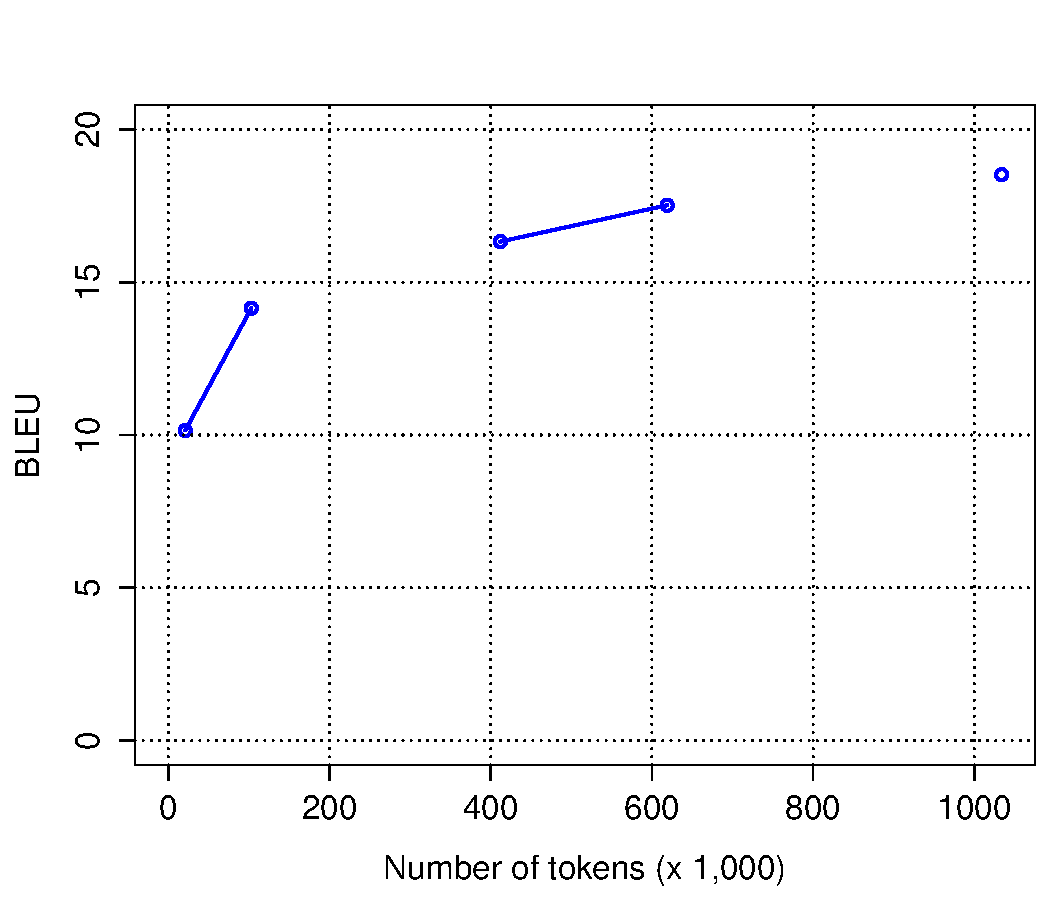
\includegraphics[width=\linewidth]{../figures/learning/learning.pdf}
%\caption{Performance of the Moses pipeline ({\bf A.A}) vs. the size of the training data (20 thousand though 1 million tokens of the Spanish-English Europarl).}
%\label{fig:learning}
%\end{center}
%\vskip -0.2in
%\end{figure}



%\subsection{Truly independent monolingual corpora} \label{sect:exp:indep}

%We now turn to estimating monolingual features from truly independent monolingual corpora we collected from web crawls for a pair of unrelated languages, Urdu (a true low-resource language) and English.  While we cannot recover as much of the lost performance (see \figref{fig:urdu}) as we did in the idealized setup of the Spanish-English experiments, the monolingual features take us a long way toward inducing a reasonable model.  We show that it is possible to estimate features using \emph{completely independent monolingual corpora}.% brings us to within 7 BLEU points of the standard bilingually estimated model. %Monolingual corpora are more plentiful than parallel data, and we expect system performance to improve further with more available data.

%\begin{figure}[t]
%\vskip -0.11in
%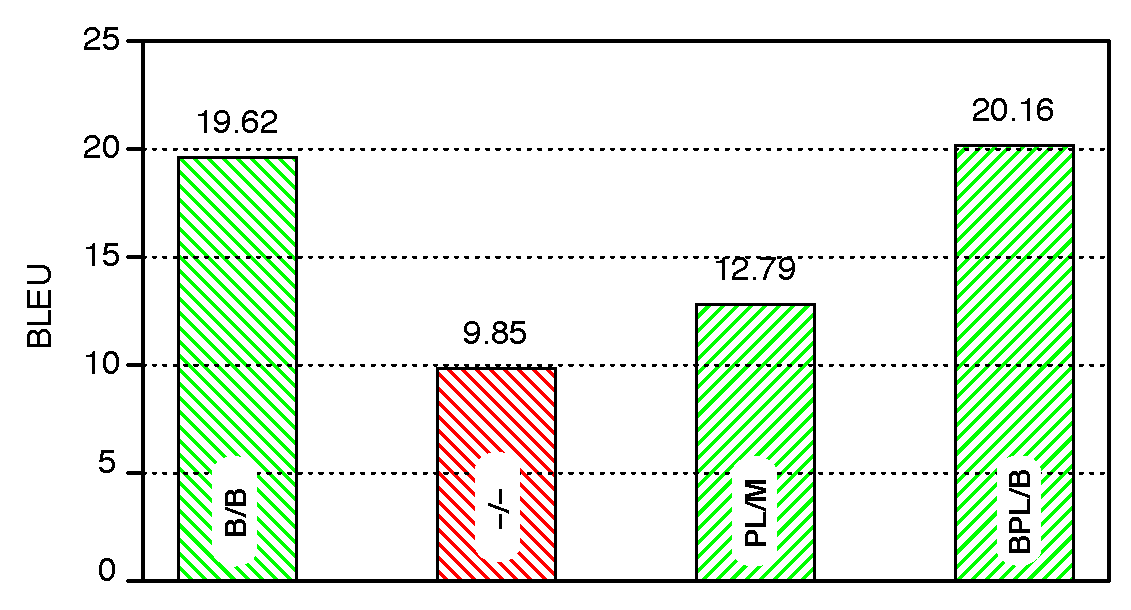
\includegraphics[width=\linewidth]{../figures/urdu/urdulegendanni.pdf}
%\caption{Performance in English-Urdu experiments, where monolingual parameters are estimated from truly  monolingual data. See \figref{fig:lesionreplacement} for key.}
%\label{fig:urdu}
%\end{figure}

%\subsection{Single language}

%\begin{enumerate}
%\item {\em Phrase features}.  (a) Augment phrase scores with mono features.  If we see better performance, reduce the amount of parallel data until it matches the performance of the original system.  Make the tradeoff argument.  (b) ({\bf lesion experiments}) See how well we do with mono features alone.
%\item {\em Orientation features}. Use mono orientation features.
%\item {\em Induce phrase table}.
%\item {\em Put everything together}.  Run the entire pipeline.
%\end{enumerate}

%\subsection{Big experiment}

%Now, run the entire pipeline on a handful of languages extracting monolingual features from the Gigaword and our crawls.

% ------------------------------------------------

% \section{Discussion} \label{sect:disc}

% ------------------------------------------------

\section{Future Work} \label{sect:conc}

%In the future we plan to build complete systems for low resource languages. In the case that very little or no parallel text is available, we expect to significantly outperform state-of-the-art MT. We have been actively collecting newswire data for many languages, which we will use to build phrase tables and estimate monolingual features, and we will make this available to the research community.

%In moving from Spanish--English translation to translation from other, less-similar languages, we expect to face new challenges. Estimating orientation probabilities, for example, for languages with very different grammars may demand a more sophisticated algorithm. However, our work here lays the foundation for this important future work.

%In this work, we use abundant monolingual data to induce a full end-to-end machine translation system, reducing the dependence on the expensive and scarce parallel texts required by state-of-the-art SMT. % We demonstrate empirically that monolingual data can get us a long way toward high quality machine translation. 
%Specifically, we define monolingual equivalents of the phrase-based translation model parameters and demonstrate that they are capable of recovering over 80\% of the performance of the standard phrase based machine translation system.  %Next, we propose several methods to induce a phrase table and show that the resulting end-to-end system significantly improves over the sole comparable past approach.  Finally, we show that monolingual data takes us a long way toward inducing a good translation model for a true low-resource language (Urdu).

%This work presents a promising direction for reducing the expensive and sparse parallel data that is assumed by state-of-the-art SMT.  
%It remains to be seen if increasing the amount of monolingual data that we use will afford continuous improvements, or if we need a more complex translation model. 

There are many interesting questions and directions for future work.  First, we plan to develop methods for inducing a phrase table, which we assumed to be given in this work. Additionally, utilizing small bitexts in combination with our monolingual parameter estimation techniques is a realistic resource condition and may improve performance further. We will investigate the relative value of bilingual and monolingual texts. %We will also explore using richer feature sets and more principled methods for constructing the phrase table. For example, when extracting phrase tables, rather than heuristically pruning the space of possible phrase pairs before scoring them, we will use approximate scoring techniques, such as Locality Sensitive Hashing \cite{Charikar2002,VanDurme2010} in order to consider a large space of potential phrase pairs.

%CONDENSED ABOVE FOR SPACE When extracting phrase tables in \secref{sect:extract}, we resorted to pruning the space of possible phrase translations before scoring them, because considering the entire space of phrase pairs is computationally infeasible.  However, relying less on pruning heuristics and being able to consider more pairs is likely to lead to better phrase tables.  Approximate scoring techniques, such as Locality Sensitive Hashing \cite{Charikar2002,VanDurme2010} would enable us to substantially expand the space of candidates we could feasibly consider.

%Named Entities are problematic for MT in general and for our setting in particular, since they tend to have low corpus counts and thus unreliable similarity scores. 

%In addition to proving to be competitive in {\it replacing} elements of the standard phrase-based MT pipeline, we have shown that using features derived from monolingual data to {\it augment} MT systems significantly improves performance. Simply adding our monolingual features to the phrase table results in over a BLEU point performance increase.

%\begin{itemize}
%\item Show that simply adding mono features => over a BLEU point gain.
%\item We plan to run this on real data for low resource languages.  We are have been actively collecting newswire data, which we plan to make available to the community.
%\item Language pairs with different writing system: use transliteration for edit distance features (as suggested in \secref{sect:phrasalfeats}).
%\item Showed that augmenting standard pipeline with monolingual features helps.
%\item Demonstrated that monolingual features are informative enough on their own for a competitive system.
%\item Proposed an algorithm for estimating orientation probabilities from monolingual data alone.
%\item Build complete systems for X low-resource languages.
%\end{itemize}

%\section*{Acknowledgments}
%The authors would like each other and their parents.

%\newpage
\bibliographystyle{acl}
% you bib file should really go here 
\bibliography{lowresmt}

\end{document}
